%----------------------------------------------------------------------------------------
%    PACKAGES AND THEMES
%----------------------------------------------------------------------------------------
\documentclass[aspectratio=169,xcolor=dvipsnames]{beamer}
\makeatletter
\def\input@path{{theme/}}
\makeatother
\usetheme{CleanEasy}
\usepackage[utf8]{inputenc}
\usepackage{lmodern}
\usepackage[T1]{fontenc}
% \usepackage[brazil]{babel}
\usepackage{fix-cm}
\usepackage{amsmath}
\usepackage{mathtools}
\usepackage{listings}
\usepackage{xcolor}
\usepackage{hyperref}
\usepackage{graphicx} % Allows including images
\usepackage{booktabs} % Allows the use of \toprule, \midrule and \bottomrule in tables
\usepackage{tikz}
\usetikzlibrary{positioning, shapes, arrows, calc, decorations.pathreplacing, arrows.meta, backgrounds, patterns, overlay-beamer-styles}
\usepackage{etoolbox}
\usepackage{animate}
\usepackage{multimedia}


\newcommand{\bx}{\mathbf{x}}
\newcommand{\by}{\mathbf{y}}
\newcommand{\pd}{p_\text{data}}
\newcommand{\pt}{p_\theta}
\newcommand{\nbx}{\nabla_{\bx}}

\newcommand{\btx}{\mathbf{\tilde{x}}}
\newcommand{\qs}{q_{\sigma}}
\newcommand{\nbtx}{\nabla_{\btx}}

%----------------------------------------------------------------------------------------
%    LAYOUT CONFIGURATION
%----------------------------------------------------------------------------------------
\input{configs/configs}
%----------------------------------------------------------------------------------------
%    TITLE PAGE
%----------------------------------------------------------------------------------------


%---------------------------------------------


\title[Diffusion models for simulations]{Diffusion models for particle physics simulations}

\author[]{Arjun Sharma}

\vspace{-2cm}\date{May 15, 2025}


%----------------------------------------------------------------------------------------


\begin{document}

\begin{frame}[plain]
  \titlepage
\end{frame}

\begin{frame}[plain]{Contents}
  \tableofcontents
\end{frame}

\section{Particle physics simulations}
\begin{frame}{}
  
\end{frame}

\section{Diffusion Models}
\begin{frame}{Generative modeling from PDFs}

Given: $\bx_1, \bx_2, \dots \bx_N$ from $p_\text{data}(\bx)$
\vspace{0.25cm}

Learn $f_\theta$ s.t.
\begin{align*}
    p_{\theta}(\bx) &= \frac{e^{f_\theta(\bx)}}{Z_\theta}\\
    \textcolor{red}{Z_\theta} &= \textcolor{red}{\int e^{f_\theta(\bx)} \,d\bx}
\end{align*}

\end{frame}

\begin{frame}{Score functions}
  \begin{columns}
    \begin{column}{0.5\textwidth}
      \[
    p_{\theta}(\bx) = \frac{e^{f_\theta(\bx)}}{Z_\theta}
    \]
    \begin{align*}
      \nbx \log \pt (\bx) &= \nbx f_\theta(\bx) - \nbx \log Z_\theta\\
                          &= \nbx f_\theta(\bx) = s_\theta(\bx)
    \end{align*}
    \end{column}
    \begin{column}{0.5\textwidth}
      \begin{figure}
      \centering
      \includegraphics[width=\textwidth]{figs/gen/gaussian_mixture_score.png}
     \end{figure}
    \end{column}
  \end{columns}
\end{frame}

\begin{frame}{Sampling with Langevin dynamics}
  \begin{columns}
    \begin{column}{0.5\textwidth}
      \begin{align*}
        \bx_{t+1} &= \bx_{t} + \alpha \cdot s_\theta(\bx_t) + \textcolor{teal}{\alpha \epsilon \cdot \mathbf{z}_t} \\
        x_0 &\sim \pi_{\text{init}}\\
        \textcolor{teal}{\textbf{z}_t} &\textcolor{teal}{\sim \mathcal{N}(0, 1)}\\
        t &= 0, 1, \dots T \to \infty
      \end{align*}
    \end{column}
    \begin{column}{0.5\textwidth}
      \centering
      \begin{figure}
        \centering
        \includegraphics[width=\textwidth]{figs/gen/gaussian_mixture_score_init.png}
      \end{figure}
    \end{column}
  \end{columns}
\end{frame}

\begin{frame}{Training objective for score}
\begin{align*}
      \mathcal{L}_\text{ESM} (\theta) &= \frac{1}{2}\mathbb{E}_{p_\text{data}(\bx)} \left[ || \textcolor{red}{\nbx \log p_\text{data}(\bx)} - s_\theta(\bx) ||_2^2\right]\\
      \iff \mathcal{L}_\text{ISM}(\theta) &= \frac{1}{2}\mathbb{E}_{p_\text{data}(\bx)} \left[ s_\theta(\bx)^2\right] + \mathbb{E}_{p_\text{data}(\bx)}\left[\nbx s_\theta(\bx) \right]\\
      \approx & \frac{1}{N} \sum\limits_{i=1}^{N}  \left[\frac{1}{2} s_\theta(\bx_i)^2 + \nabla_{\bx_i} s_\theta(\bx_i)  \right]
  \end{align*}
\end{frame}

\begin{frame}{Drawbacks}
  \begin{columns}
    \begin{column}{0.4\textwidth}
      \centering
      Field in low-density regions
    \end{column}
    \begin{column}{0.6\textwidth}
      \centering
      Scaling
    \end{column}
  \end{columns}

  \begin{columns}
    \begin{column}{0.4\textwidth}
      \centering
      \begin{figure}
        \centering
        \includegraphics[height=0.32\textheight]{figs/gen/score_field_training_0.png}
      \end{figure}

        \begin{figure}
          \centering
        \includegraphics[height=0.32\textheight]{figs/gen/score_field_training_final}
      \end{figure}
    \end{column}
    \begin{column}{0.6\textwidth}
      \centering
      \begin{align*}
        &\frac{1}{2}\mathbb{E}_{p_\text{data}(\bx)} \left[ s_\theta(\bx)^2\right] + \mathbb{E}_{p_\text{data}(\bx)}\left[\nbx s_\theta(\bx) \right]
      \end{align*}
      
      \rule{0.8\textwidth}{0.4pt}
      
      \begin{align*}
        \underset{
          \textcolor{teal}{\text{Forward propagation}}
        }{ \frac{1}{2}\mathbb{E}_{p_\text{data}(\bx)} \left[ s_\theta(\bx)^2\right]} 
        + \underset{
          \textcolor{red}{\text{Backprops}~\propto~\text{dim}(\bx)}
        }{\mathbb{E}_{p_\text{data}(\bx)}\left[\text{trace}(\nbx s_\theta(\bx)) \right]}
      \end{align*}
    \end{column}
  \end{columns}
\end{frame}


\begin{frame}{Noise perturbation}

\begin{align*}
  \btx &= \bx + z\\
  z &\sim \mathcal{N}(0, 1)\\
    \qs(\btx | \bx) &= \mathcal{N}(\bx, \sigma^2 I)
  \end{align*}
\end{frame}

\begin{frame}{Denoising objective}
  \begin{align*}
    \mathcal{L}_{\text{ESM} \sigma}(\theta, \sigma) &= \frac{1}{2} \mathbb{E}_{\qs(\btx)} \left[|| s_\theta(\btx) - \nbtx \log q_\sigma(\btx) ||_2^2 \right]\\
    \iff \mathcal{L}_{\text{ISM} \sigma}(\theta, \sigma) &= \frac{1}{2} \mathbb{E}_{\qs(\btx, \bx)} \left[ ||s_\theta(\btx) - \nbtx \log q_{\sigma} (\btx | \bx) ||_2^2 \right]
  \end{align*}
\end{frame}

\begin{frame}{Gradient of the corrupted distribution}
  \begin{align*}
    \nbtx \log \qs (\btx | \bx) &= \nbtx \log \frac{1}{(2\pi)^{\frac{d}{2}}  \sigma^d} e^{-\frac{1}{2 \sigma^2} || \btx - \bx||^2}\\
                        &= \nbtx \log e^{-\frac{1}{2 \sigma^2} || \btx - \bx||^2} - \nbtx \log (2\pi)^{\frac{d}{2}} \sigma^d\\
                        &= - \nbtx \frac{1}{2 \sigma^2} || \btx - \bx||^2\\
                        &= \frac{|| \btx - \bx||}{\sigma^2}\\
    \therefore \mathcal{L}_{\text{ISM} \sigma}(\theta, \sigma) &= \frac{1}{2} \mathbb{E}_{\qs(\btx, \bx)} \left[ ||s_\theta(\btx) -  \frac{|| \btx - \bx||}{\sigma^2} ||_2^2 \right]
  \end{align*}
\end{frame}

\begin{frame}{Multiple noise levels}

  \begin{columns}
    \begin{column}{0.32\textwidth}
      \includegraphics[width=0.8\textwidth]{figs/gen/mixture_with_noise_0.0.png}
    \end{column}
      \begin{column}{0.32\textwidth}
      \includegraphics[width=0.8\textwidth]{figs/gen/mixture_with_noise_0.01.png}
    \end{column}
    \begin{column}{0.32\textwidth}
      \includegraphics[width=0.8\textwidth]{figs/gen/mixture_with_noise_0.1.png}
    \end{column}
  \end{columns}

  \begin{columns}
      \begin{column}{0.32\textwidth}
      \includegraphics[width=0.8\textwidth]{figs/gen/mixture_with_noise_0.5.png}
    \end{column}
      \begin{column}{0.32\textwidth}
      \includegraphics[width=0.8\textwidth]{figs/gen/mixture_with_noise_1.0.png}
    \end{column}
        \begin{column}{0.32\textwidth}
      \includegraphics[width=0.8\textwidth]{figs/gen/mixture_with_noise_2.0.png}
    \end{column}
  \end{columns}
  
\end{frame}

\begin{frame}{Multiple noise levels}
  
  \begin{align*}
    \mathcal{L} (\theta, \{ \sigma_i \}_{i=1}^L) &= \frac{1}{L} \sum\limits_{i=1}^L \textcolor{teal}{\lambda(\sigma_i)} \mathbb{E}_{q_{\sigma_i} (\btx, \bx)} \left[ ||s_\theta(\btx, \textcolor{teal}{\sigma_i}) -  \frac{|| \btx - \bx||}{\sigma^2} ||_2^2 \right]
  \end{align*}
\end{frame}

\begin{frame}{Sampling with annealed Langevin dynamics}
  \begin{align*}
    \btx_0 &\sim \pi_\text{init}\\
  \end{align*}
  From $i = 1, 2, \dots L$ with $\frac{\sigma_1}{\sigma_2} = \cdots = \frac{\sigma_{L-1}}{\sigma_L} > 1$
  \begin{align*}
    \alpha_i &= \gamma \frac{\sigma_i^2}{\sigma_L^2}\\
    \btx_t &= \btx_{t-1} + \alpha_i s_\theta(\btx_{t-1}, \sigma_i) + \epsilon \alpha_i \mathbf{z}_t\\
    \mathbf{z}_t &\sim \mathcal{N}(0, 1)
  \end{align*}
\end{frame}

\begin{frame}{Conditional generation}
  \begin{align*}
   p(\bx | \by) &= \frac{p(\by | \bx) p(\bx)}{\textcolor{red}{p(\by)}}
  \end{align*}
  \begin{align*}
    \nbx \log p(\bx | \by) &= \nbx \log p(\by | \bx) + \nbx \log p(\bx) - \nbx \log p(\by)\\
                           &= \nbx \log p(\bx) + \nbx \log p(\by | \bx) \\
                           &= \textcolor{teal}{s_\theta(\bx)} + \textcolor{olive}{\gamma} \nbx \log p(\by | \bx)
  \end{align*}
\end{frame}

\begin{frame}{Single model for guidance}
  \begin{align*}
    p(\by | \bx) &= \nbx \log p(\bx | \by) - \nbx \log p(\bx)\\
    \implies  \nbx \log p(\bx | \by) &= \nbx \log p(\bx) + \gamma \nbx \log p(\bx | \by) - \gamma \nbx \log p(\bx) \\
                                     &= \gamma \nbx \log p(\bx | \by) + (\gamma - 1)  \nbx \log p(\bx)\\
                                     &\textcolor{teal}{\approx \gamma s_\theta(\bx, \by) - (\gamma - 1) s_\theta(\bx, \phi)}
  \end{align*}
\end{frame}

\section{Equivariant learning}
\begin{frame}{Definitions}
  
\end{frame}

\begin{frame}{Equivariant diffusion models}
  
\end{frame}


\begin{frame}{Lorentz equivariance}
  
\end{frame}

\begin{frame}{Lorentz-equivariant learning}

\end{frame}

\section{Appendices}

\begin{frame}{Artificial neuron}

\begin{columns}
  \begin{column}{0.75\textwidth}
    \centering
    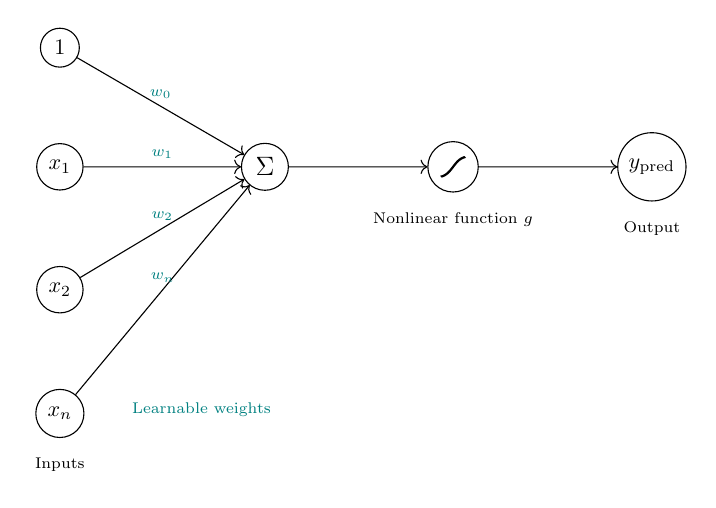
\begin{tikzpicture}[
      scale=0.8, transform shape,
      node distance=1.2cm and 1.8cm,
      input/.style={circle, draw, minimum size=0.6cm},
      sum/.style={circle, draw, minimum size=0.6cm, font=\large},
      nonlin/.style={circle, draw, minimum size=0.8cm},
      output/.style={circle, draw, minimum size=0.6cm}
    ]

    % Input nodes
    \node[input] (c) {$1$};
    \node[input, below=of c] (x1) {$x_1$};
    \node[input, below=of x1] (x2) {$x_2$};
    \node[input, below=of x2] (xn) {$x_n$};

    % Summation node
    \node[sum, right=2.5cm of x1] (sum) {$\Sigma$};

    % Nonlinearity node
    \node[nonlin, right=2.2cm of sum] (nonlin) {};

    % Draw sigmoid inside nonlinearity node
    \begin{scope}
      \clip (nonlin) circle(0.25cm); % Clip to circle around nonlin node
      \begin{scope}[shift={(nonlin.center)}] % Shift plot so (0,0) is at center of nonlin
        \draw[domain=-2:2, variable=\x, samples=100, thick]
          plot ({\x*0.2}, {0.35/(1 + exp(-3*\x)) - 0.175});
      \end{scope}
    \end{scope}

    % Output node
    \node[output, right=2.2cm of nonlin] (out) {$y_{\text{pred}}$};

    % Arrows from inputs to sum node
    \draw[->] (c) -- node[above] {\scriptsize \textcolor{teal}{$w_0$}} (sum);
    \draw[->] (x1) -- node[above] {\scriptsize \textcolor{teal}{$w_1$}} (sum);
    \draw[->] (x2) -- node[above] {\scriptsize \textcolor{teal}{$w_2$}} (sum);
    \draw[->] (xn) -- node[above] {\scriptsize \textcolor{teal}{$w_n$}} node[pos=0.0, below, xshift=2cm] {\scriptsize \textcolor{teal}{Learnable weights}} (sum);

    % Arrows between processing stages
    \draw[->] (sum) -- (nonlin);
    \draw[->] (nonlin) -- (out);

    % Label below nonlinearity
    \node[below=0.2cm of xn] {\scriptsize Inputs};
    \node[below=0.2cm of nonlin] {\scriptsize Nonlinear function $g$};
    \node[below=0.2cm of out] {\scriptsize Output};

  \end{tikzpicture}

  \end{column}
  \begin{column}{0.25\textwidth}
    \[
    y_\text{pred} = g(w_0 + \mathbf{w}^T \cdot \mathbf{x})
    \]
  \end{column}
\end{columns}
\end{frame}


\begin{frame}{Derivation of divergence objective for score}
  \small
  \begin{align*}
    &\frac{1}{2}\mathbb{E}_{p_\text{data}(\bx)} \left[ || \textcolor{red}{\nbx \log p_\text{data}(\bx)} - s_\theta(\bx) ||_2^2\right]\\
    &= \frac{1}{2} \int p_\text{data}(\bx) \left(\textcolor{red}{\nbx \log p_\text{data}(\bx)} - \nbx f_\theta(\bx) \right)^2 \,d\bx\\
    &= \underset{\textcolor{teal}{{\text{Constant in training}}}}{\frac{1}{2} \int p_\text{data}(\bx) \left(\textcolor{red}{\nbx \log p_\text{data}(\bx)}\right)^2 \,d\bx
    }+ \frac{1}{2} \int p_\text{data}(\bx) \left(\nbx f_\theta(\bx) \right)^2 \,d\bx - \underset{
    \textcolor{teal}{\text{Use }\nbx \log p_\text{data}(\bx) = \frac{\nbx p_\text{data}(\bx)}{p_\text{data}(\bx)}}  
    }
    {\int p_\text{data}(\bx) \textcolor{red}{\nbx \log p_\text{data}(\bx)} \cdot \nbx f_\theta(\bx) \,d\bx}\\
    &= C + \frac{1}{2} \int p_\text{data}(\bx) \left(\nbx f_\theta(\bx) \right)^2 \,d\bx - \underset{\textcolor{teal}{\text{Integrate by parts}}}{\int \textcolor{red}{\nbx p_\text{data}(\bx)}  \cdot \nbx f_\theta (\bx) \,d \bx}\\
    &=  C + \frac{1}{2} \int p_\text{data}(\bx) \left(\nbx f_\theta(\bx) \right)^2 \,d\bx - \underset{\textcolor{teal}{\text{Boundary values } \to~ 0}}{p_\text{data}(\bx) \nabla_x f_\theta(\bx)|_{-\infty}^{\infty}}  + \int p_\text{data}(\bx) \nbx \nbx f_\theta(\bx) d \bx\\
    &= C + \frac{1}{2} \mathbb{E}_{p_\text{data}(\bx)} \left[\nbx f_\theta(\bx)^2\right] +\mathbb{E}_{p_\text{data}(\bx)} \left[ \nbx^2 f_\theta(\bx)\right] = C + \frac{1}{2}\mathbb{E}_{p_\text{data}(\bx)} \left[ s_\theta(\bx)^2\right] + \mathbb{E}_{p_\text{data}(\bx)}\left[\nbx s_\theta(\bx) \right]
  \end{align*}
\end{frame}

\begin{frame}{Derivation of noise-perturbed divergence objective}
  \small
  \begin{align*}
    &\frac{1}{2} \mathbb{E}_{q_\sigma(\btx)} \left[ || s_\theta(\btx) - \textcolor{red}{\nbtx \log q_\sigma (\btx)} ||_2^2 \right]\\
    =&\frac{1}{2} \mathbb{E}_{q_\sigma(\btx)} \left[ s_\theta(\btx)^2 \right] - \underset{\textcolor{teal}{\text{Use}~\nbtx \log q_\sigma (\btx) = \frac{\nbtx q_\sigma(\btx)}{q_\sigma(\btx)} }}{ \int q_{\sigma}(\btx) s_\theta(\btx) \nbtx \log q_\sigma(\btx)  \,d \btx} + \underset{\textcolor{teal}{\text{Constant in training}}}{\frac{1}{2} \int q_\sigma (\btx) (\textcolor{red}{\nbtx \log q_\sigma(\btx)})^2 \,d\btx}\\
    &\underset{\textcolor{teal}{\text{Use } q_\sigma(\btx) = \int p_\text{data}(x) p_\sigma(\btx | bx)} }{ \int s_\theta(\btx) \textcolor{red}{\nbtx q_\sigma(\btx)}  \,d \btx}\\
    = &\underset{\text{\textcolor{teal}{Differentiation under integral}}}{\int s_\theta(\btx) \nbtx \left( \int p_\text{data} (\bx) q_\sigma(\btx | \bx) \,d \bx \right) \, d \btx}  \\
    =& \underset{\textcolor{teal}{\text{Use } \nbtx q_\sigma(\btx | \bx) = q_\sigma (\btx | \bx) \nbtx \log q_\sigma(\btx | \bx)}}{\int s_\theta(\btx) \left( \int p_\text{data}(\bx) \nbtx q_\sigma(\btx | \bx) \,d \bx \right) \,d \btx } = \int \int s_\theta(\btx)  p_\text{data}(\bx) q_\sigma (\btx | \bx) \nbtx \log q_\sigma(\btx | \bx) \,d \bx \,d \btx \\
    =& \mathbf{E}_{q_\sigma(\btx, \bx)} \left[ s_\theta(\btx) \nbtx \log q_\sigma(\btx | \bx) \right]
  \end{align*}
\end{frame}



\begin{frame}{U-Net}
  \centering
  \begin{figure}
    \includegraphics[height=0.65\textheight]{figs/unet-Ronneberger2015.png}
  \end{figure}
  \tiny{
        Source: Ronneberger et al. (2015)
  }
\end{frame}



% \begin{frame}{Diffusion models as SDEs}
  
% \end{frame}


% \begin{frame}{Lists and Numbering}
%   \begin{columns}
%     \begin{column}{0.48\textwidth}
%       Bulleted list:
%       \begin{itemize}
%         \item First level item
%         \begin{itemize}
%           \item Second level item
%           \item Another second level
%           \begin{itemize}
%             \item Third level item
%           \end{itemize}
%         \end{itemize}
%         \item Another first level item
%       \end{itemize}
%     \end{column}
%     \begin{column}{0.48\textwidth}
%       Numbered list:
%       \begin{enumerate}
%         \item First step
%         \begin{enumerate}
%           \item Substep one
%           \item Substep two
%         \end{enumerate}
%         \item Second step
%         \item Third step
%       \end{enumerate}
%     \end{column}
%   \end{columns}
% \end{frame}



\end{document}